\documentclass[10pt, letterpaper]{report}
% !TeX program = xelatex
%==================PREAMBOLO=======================%
\usepackage[utf8]{inputenc}
\usepackage{psvectorian}
\usepackage{pgfplots}
\usepackage[Rejne]{fncychap}
\usepackage[export]{adjustbox}
\usepackage[T1]{fontenc}
\usepackage{lmodern}
\usepackage{blindtext}
\usepackage{pdfpages}
\usepackage[shortlabels]{enumitem}
\usepackage{moresize}
\usepackage{graphicx} % Required for inserting images
\usepackage{hyperref}
\usepackage{listings}
\usepackage[table,xcdraw]{xcolor}
\usepackage{amssymb}
\usepackage{amsmath}
\usepackage[italian]{babel}
\usepackage{nicefrac, xfrac}
\usepackage{tikz}
\usepackage{tikz-3dplot}
\usepackage{mathrsfs} 
\usepackage{titletoc}
\usepackage{fancyhdr}
\usepackage{psvectorian,lipsum}
\usepackage{fourier-orns}
\usepackage{lipsum}
\usepackage{multicol}
\usepackage[paper=a4paper,left=25mm,right=25mm,bottom=25mm,top=25mm]{geometry}
\definecolor{light-gray}{gray}{0.95}
\definecolor{cop}{HTML}{f7ecd7}
\definecolor{copAut}{HTML}{ababab}
\definecolor{copAut2}{HTML}{c3c3e6}
\definecolor{purcop}{HTML}{d0d3db}
\definecolor{sapienza}{HTML}{660f1d}
\definecolor{lightSapienza}{HTML}{e3d3d5}
\definecolor{darkgreen}{HTML}{008000}
\definecolor{cartaRiciclata}{HTML}{fcfcf7}
\newcommand{\redText}[1]{\color{red}#1\color{black}}
\newcommand{\code}[1]{\colorbox{light-gray}{\texttt{#1}}}
\newcommand{\codee}[1]{\colorbox{white}{\texttt{#1}}}
\newcommand{\K}{{\mathbb K}}
\newcommand{\notimplies}{%
  \mathrel{{\ooalign{\hidewidth$\not\phantom{=}$\hidewidth\cr$\implies$}}}}
\newcommand{\flowerLine}{ \begin{center}\decofourleft\hphantom{ }\decoone\hphantom{ }\decofourright\hphantom{}\hphantom{aa}
\decofourleft\hphantom{ }\decoone\hphantom{ }\decofourright\hphantom{}\hphantom{aa}
\decofourleft\hphantom{ }\decoone\hphantom{ }\decofourright\hphantom{}\hphantom{aa}
\decofourleft\hphantom{ }\decoone\hphantom{ }\decofourright\hphantom{}\hphantom{aa} 
\decofourleft\hphantom{ }\decoone\hphantom{ }\decofourright\hphantom{}\hphantom{aa}
\decofourleft\hphantom{ }\decoone\hphantom{ }\decofourright\hphantom{}\hphantom{aa}
\decofourleft\hphantom{ }\decoone\hphantom{ }\decofourright\hphantom{}\hphantom{aa}
\decofourleft\hphantom{ }\decoone\hphantom{ }\decofourright\hphantom{}\hphantom{aa}
\decofourleft\hphantom{ }\decoone\hphantom{ }\decofourright\hphantom{}\hphantom{aa}
\end{center}}
\definecolor{g}{RGB}{60, 50, 50}
\newcommand{\textg}[1]{\color{g}{\textbf{#1}}\color{black}}
\newcommand{\teo}[1]{{\large\color{sapienza}\textbf{Teorema #1 :\hphantom{a}}}}
\newcommand{\defi}[1]{{\large\color{sapienza}\textbf{Definizione #1 :\hphantom{a}}}}
\newcommand{\claim}[1]{{\color{sapienza}\textbf{Claim #1 :\hphantom{a}}}}
\newcommand{\lemma}[1]{{\color{sapienza}\textbf{Lemma #1 :\hphantom{a}}}}
\newcommand{\dimo}[1]{{\color{sapienza}\textbf{Dimostrazione #1 :\hphantom{a}}}}
\newcommand{\prop}[1]{{\color{sapienza}\textbf{Proposizione #1 :\hphantom{a}}}}
\newcommand\greybox[1]{%
  \vskip\baselineskip%
  \par\noindent\colorbox{light-gray}{%
    \begin{minipage}{\textwidth}#1\end{minipage}%
  }%
  \vskip\baselineskip%
}
\newcommand\sapbox[1]{%
  \vskip\baselineskip%
  \par\noindent\colorbox{lightSapienza}{%
    \begin{minipage}{\textwidth}#1\end{minipage}%
  }%
  \vskip\baselineskip%
}
\newcommand{\ridFunc}{{f:\Sigma^*\rightarrow \Sigma^*}}
\newcommand{\rid}{{\le_m^P}}
\newcommand{\Z}{{\mathbb Z}}
\newcommand{\blank}{{\sqcup}}
\newcommand{\R}{{\mathbb R}}
\newcommand{\N}{{\mathbb N}}
\newcommand{\C}{{\mathbb C}}
\newcommand{\Sn}{{\mathcal S_n}}
\newcommand{\An}{{\mathcal A_n}}
\newcommand{\E}{{\mathcal E}}
\newcommand{\B}{{\mathcal B}}
\newcommand{\mcm}{{\text{mcm}}}
\newcommand{\rg}{{\text{rg}}}
\newcommand{\ve}{{\bar v}}
\newcommand{\spaz}{{\text{\hphantom{aa}}}}
\newcommand{\MCD}{{\text{MCD}}}
\newcommand{\tc}{{\text{ tale che }}}
\newcommand{\supp}{{\text{Supp}}}
\newcommand{\acc}{\\\hphantom{}\\}
\newcommand{\esempio}[1]{{\acc\large\color{sapienza}\textbf{Esempio #1 \hphantom{a}}\acc}}
\newcommand{\bra}[1]{\langle #1 \rangle}
\newcommand{\aut}{{\text{Aut}}}
\newcommand{\Span}{{\text{Span}}}
\newcommand{\End}{{\text{End}}}
\newcommand{\cen}{{\text{Centro}}}
\newcommand{\norm}{{\unlhd}}
\newcommand{\ciclS}{{\left \langle }}
\newcommand{\ciclE}{{\right \rangle }}
\newcommand{\boxedMath}[1]{\begin{tabular}{|c|}\hline \texttt{#1} \\ \hline\end{tabular} :} 
\newcommand{\shell}[1]{\colorbox{black}{\textcolor{white}{\texttt{#1}}}}
\newcommand{\eqImportante}[1]{\begin{center}\huge\lefthand\hphantom{a}
    \normalsize\texttt{#1}
    \hphantom{aaa}\huge\righthand\end{center}}

\fancyhf{}
\pagestyle{fancy}
\usepackage{pgf-pie}  
\usetikzlibrary{positioning}

\renewcommand{\headrule}{%
\vspace{-8pt}\hrulefill
\raisebox{-2.1pt}{\quad\decothreeleft\decotwo\decothreeright\quad}\hrulefill}

%sta roba serve per il codice C
\definecolor{mGreen}{rgb}{0,0.6,0}
\definecolor{mGray}{rgb}{0.5,0.5,0.5}
\definecolor{mPurple}{rgb}{0.58,0,0.82}
\definecolor{backgroundColour}{rgb}{0.95,0.95,0.92}

\lstdefinestyle{CStyle}{
    backgroundcolor=\color{backgroundColour},   
    commentstyle=\color{mGreen},
    keywordstyle=\color{magenta},
    numberstyle=\tiny\color{mGray},
    stringstyle=\color{mPurple},
    basicstyle=\footnotesize,
    breakatwhitespace=false,         
    breaklines=true,                 
    captionpos=b,                    
    keepspaces=true,                 
    numbers=left,                    
    numbersep=5pt,                  
    showspaces=false,                
    showstringspaces=false,
    showtabs=false,                  
    tabsize=2,
    language=C
}
\lstdefinestyle{CppStyle}{
    backgroundcolor=\color{backgroundColour},   
    commentstyle=\color{mGreen}\ttfamily,
    morecomment=[l][\color{magenta}]{\#}
    keywordstyle=\color{blue}\ttfamily,
    numberstyle=\tiny\color{mGray},
    stringstyle=\color{red}\ttfamily,
    basicstyle=\ttfamily,
    breakatwhitespace=false,         
    breaklines=true,                 
    captionpos=b,                    
    keepspaces=true,                 
    numbers=left,                    
    numbersep=5pt,                  
    showspaces=false,                
    showstringspaces=false,
    showtabs=false,                  
    tabsize=2,
    language=C
}
\lstset{language=C++,
                basicstyle=\ttfamily,
                keywordstyle=\color{blue}\ttfamily,
                stringstyle=\color{red}\ttfamily,
                commentstyle=\color{green}\ttfamily,
                morecomment=[l][\color{magenta}]{\#}
}
%fine roba che serve per il codice C
\usepackage{minted}
 %TOGLI COMMENTO SE USI XELATEX

\title{Calcolo Integrale} %========TITOLO========%
\author{Marco Casu}
\date{\vspace{-5ex}}
\begin{document}

%==================COPERTINA=======================%
\begin{titlepage}
    %\pagecolor{cop}
\begin{center}
    %TOGLI COMMENTO SE USI XELATEX
    %\setmainfont{Palace Script MT}\HUGE Marco Casu\acc
    %\setmainfont{Grand Casino}
     %TOGLI COMMENTO SE USI XELATEX
    %\setmainfont{h Halfroad}
    \HUGE \decothreeleft\hphantom{ }{\fontsize{48}{50}\selectfont Calcolo Integrale}\hphantom{ }\decothreeright
     %TOGLI COMMENTO SE USI XELATEX
    %\setmainfont{Times New Roman}
\end{center}
\thispagestyle{empty}
\begin{figure}[h]
    \centering{
        %l'immagine deve avere una risoluzione 2048x2048
        \includegraphics[width=1\textwidth ]{images/copertina2.jpeg}
    }
\end{figure}
\vfill 
\centering \includegraphics[width=0.4\textwidth ]{../../../../../preamble/Stemma_sapienza.png} \acc
\centering \Large \color{sapienza}Facoltà di Ingegneria dell'Informazione,
Informatica e Statistica\\
Dipartimento di Informatica
\end{titlepage}

%===================FINE COPERTINA======================%
\newpage
\pagecolor{cartaRiciclata}%\setmainfont{Algerian}\Large
Questo documento è distribuito sotto la licenza 
\color{blue}\href{https://www.gnu.org/licenses/fdl-1.3.txt}{GNU}\color{black},  
è un resoconto degli appunti (eventualmente integrati con libri di testo) tratti dalle lezioni del corso di Calcolo Integrale
\hphantom{a}per la laurea 
triennale in Informatica. Se dovessi notare errori, ti prego di segnalarmeli.



\textbf{nota bene :} questi appunti sono estremamente riassuntivi, non possono essere sostituiti 
completamente al libro di testo.
\newpage %\setmainfont{Times New Roman}
\normalsize
\tableofcontents 
\newpage

%==================FOOTER e HEADER=======================%
\fancyhf{}
\fancyhead[L]{\nouppercase{\leftmark}}
\fancyhead[R]{Sezione \thesection}
\fancyfoot[C]{\thepage}
\fancyfoot[L]{Appunti di Calcolo Integrale}
\fancyfoot[R]{Marco Casu }
%==================FOOTER e HEADER=======================%

%Ricorda del comando \flowerLine per separare le sottosezioni. Le sezioni si separano nelle diverse pagine

%==================INIZIO======================%




\chapter{Serie numeriche}
\defi{} Una serie numerica, è una successione costruita a partire da altre successioni. Il valore 
$n$-esimo è la somma di tutti i valori precedenti della successione.
$$ S_n = \sum_{k=0}^n a_k\text{ con }n\in \Z^+$$ 
Ad esempio
$$ a_n=n^2\implies S_3 = 0^2+1^2+2^2+3^2=14$$
\section{Convergenza}
La somma molto spesso viene valutata per $n$ che tende all'infinito, un altro esempio di serie 
numerica è il seguente 
$$ \sum_{k=0}^\infty \dfrac{1}{k+1}=1+\frac{1}{2}+\frac{1}{3}+\dots$$
Una serie numerica viene caratterizzata dalla sua \textit{convergenza}.\acc 
\defi{}Una serie numerica $S_n$ si dice \textbf{convergente} se 
$$ \lim_{n\rightarrow \infty} S_n = l$$
Si scrive anche 
$$S_n =\displaystyle \sum_\text{k=0}^n a_k < \pm\infty$$
Diversamente, se la somma degli infiniti termini della serie vale $\pm\infty$, 
la serie si dice \textit{divergente}, un classico esempio di serie divergente è il seguente 
$$ \sum_{k=1}^\infty k^2=1+4+9+16+25\dots = \infty$$
Infine una serie può non essere divergente, ma nemmeno convergente, ossia non è 
definito un valore alla quale converge, si dice \textit{non convergente} o 
\textit{irregolare}, un tipico esempio è 
$$ \sum_{k=1}^\infty (-1)^k=-1+1-1+1-1+1\dots $$
\subsection{Serie geometriche}
Una serie $\sum_{\infty}a_k$ si dice serie \textbf{geometrica} se 
$a_k$ è della forma $q^k$, ossia quando il valore $k$-esimo della sommatoria 
è posto come esponente ad un numero reale.\acc
\prop{} vale la seguente
$$ \sum_{k=0}^n q^k = \dfrac{q^{n+1}-1}{q-1}$$
\dimo{} Si consideri
$$ S_n =  \sum_{k=0}^n q^k = 1+q+q^2+q^3\dots + q^n$$
si moltiplicano entrambi i membri per $(1-q)$
$$\begin{matrix}
    \displaystyle(1-q)\cdot S_n =(1-q)\cdot 
     (\sum_{k=0}^n q^k = 1+q+q^2+q^3\dots + q^n) \implies  
    (1-q)\cdot S_n = 1-q^{n+1} 
\end{matrix}$$
Divido entrambi i membri per $(1-q)$
$$S_n = \dfrac{1-q^{n+1}}{(1-q)}\;\;\blacksquare$$
Considerando $q^k$, assume diversi valori per $k\rightarrow\infty$ in base 
ai valori di $q$
$$\lim_{k\rightarrow\infty} q^k=\begin{cases}
    0\text{ se }q\in (-1,1)\\ 
    1\text{ se }q=1\\
    \infty\text{ se }q>1\\
    \text{indeterminato se }q<-1
\end{cases} $$
Di una serie geometrica, è possibile stabilirne il carattere in base al 
valore di $q$, di fatto si ha che 
$$ \sum_{k=0}^\infty q^k = \begin{cases}
    0\text{ se }q=0\\ 
    \frac{1}{1-q}\text{ se }q\in (-1,1)\\
    \infty\text{ se }q\ge1\\
    \text{indeterminato se }q<-1
\end{cases}$$
\subsection{Serie armoniche}
Una serie $\sum_{\infty}a_k$ si dice serie \textbf{armonica} se il valore 
$k$-esimo della sommatoria è posto come denominatore della successione, ed è 
elevato ad un numero reale.
$$\sum_{k=0}^\infty \dfrac{1}{k^a}\;\;a\in\R$$
Se l'esponente reale $a$ è maggiore di $1$, la sommatoria converge, se invece è 
compreso fra $0$ ed $1$, diverge.
$$ \sum_{k=0}^\infty \dfrac{1}{k^a} = \begin{cases}
    l\in \R\text{ se }a>1\\ 
    \infty\text{ se }a\in [0,1]\\
\end{cases}$$
Vediamo un esempio, si vuole sapere se la serie
 $\displaystyle \sum_{k=0}^\infty \dfrac{\cos^2(k)}{k^2}$
sia divergente oppure no.
Innanzitutto, notiamo come 
 $\cos^2(k)$ sia limitato, quindi sempre minore o uguale ad $1$, come mostrato in 
 figura \ref{fig:coss}.
 \begin{figure}[h!]
    \centering
    \begin{tikzpicture}
        \begin{axis}[
            axis lines = left,
            xlabel = \(k\),
            ylabel = {\(f(k)\)},
        ]
        %Below the red parabola is defined
        \addplot [
            domain=-5:5, 
            samples=500, 
            color=red,
        ]
        {1};
        \addlegendentry{\(1\)}
        %Here the blue parabola is defined
        \addplot [
            domain=-5:5, 
            samples=500, 
            color=blue,
            ]
            {(cos(deg(x)))^2};
        \addlegendentry{\(\cos^2(k)\)}
        
        \end{axis}
        \end{tikzpicture}
    \label{fig:coss}
    \caption{coseno limitato}
\end{figure}
$$\dfrac{\cos^2(k)}{k^2}\le \dfrac{1}{k^2}
\implies 
\sum_{k=0}^\infty \dfrac{\cos^2(k)}{k^2}\le \sum_{k=0}^\infty \dfrac{1}{k^2}$$
Essendo che $\sum_{k=0}^\infty \dfrac{1}{k^2}$ converge ad un valore finito, allora
necessariamente   $$ \sum_{k=0}^\infty \dfrac{\cos^2(k)}{k^2}<\infty$$
\subsection{Teoremi sulle serie e criteri di convergenza}
In questa sezione verranno presentati alcuni teoremi fondamentali riguardo la convergenza 
delle serie. \acc 
\teo{della condizione necessaria} Sia $S_n$ una serie convergente, del tipo 
$$ S_n=  \sum_{k=0}^\infty a_k = l\in \R$$
allora $$\lim_{k\rightarrow\infty}a_k=0$$
\dimo{} 
$$\begin{matrix} 
    S_n-S_{n-1}= \sum_{k=0}^n a_k-\sum_{k=0}^{n-1} a_k =  \\
    (a_1+a_2\dots+ a_{n-1}+a_n)-(a_1+a_2\dots+ a_{n-1})=
    a_n \implies \lim_{k\rightarrow\infty}a_k=0
\end{matrix} $$
\teo{sulle serie a termini positivi}
Sia $S_n=  \sum_{k=0}^\infty a_k$, si ha che 
$$ a_k\ge 0 \;\;\forall k\implies S_n \begin{cases}
   \text{ converge}\\
    \text{ diverge a }+\infty
\end{cases}$$
\teo{del confronto} Siano $a_k$ e $b_k$ due successioni tali che $0<a_k<b_k$, allora\begin{itemize}
    \item $ \sum_{k=0}^\infty b_k<\infty \implies \sum_{k=0}^\infty a_k<\infty$
    \item $ \sum_{k=0}^\infty a_k=\infty \implies \sum_{k=0}^\infty b_k=\infty$
\end{itemize}
Consideriamo adesso due successioni  $a_k$ e $b_k$ tali che $0<a_k \land 0<b_k$ e 
$\displaystyle \lim_{k\rightarrow \infty}\dfrac{a_k}{b_k}=l$, allora \begin{itemize}
    \item $ \sum_{k=0}^\infty a_k<\infty \iff \sum_{k=0}^\infty b_k<\infty$
    \item $ \sum_{k=0}^\infty a_k=\infty \iff \sum_{k=0}^\infty b_k=\infty$
\end{itemize}
Questo teorema ci dice che, se due successioni si comportano asintoticamente allo stesso modo, 
allora le serie che le hanno come termini si comporeranno allo stesso modo riguardo 
la convergenza, e possono essere approssimate ad una stessa funzione.\acc 
Il seguente criterio è detto \textit{del rapporto e della radice}, sono in realtà 
due differenti criteri, con premesse differenti ma che espongono la stessa tesi. Sia 
$a_k\ge 0$, tale che 
$$ \lim_{k\rightarrow \infty} \dfrac{a_{k+1}}{a_k}= L\ne 1 \;\text{ oppure }\;
\lim_{k\rightarrow \infty} \sqrt[k]{a_k}= L\ne 1$$ 
allora $$\begin{cases}
   \text{la serie converge se } L\in [0,1)\\
   \text{la serie converge se } L>1
\end{cases}
 $$
 La seguente formula è detta formula di \textbf{Sterling} e descrive 
 il comportamento asintotico della funzione fattoriale, riguardo la velocità 
 della sua crescita verso infinito 
 $$ 
 \lim_{x\rightarrow \infty} \dfrac{x!}{x^xe^{-x}\sqrt{2\pi x}}=1
 $$
 \teo{del criterio di Leibniz} Si consideri una serie, in cui è presente 
 il termine $(-1)^k$, nonostante il segno non sia costante, tale criterio permette 
 di decretare la convergenza della serie. La serie in questione è del tipo 
 $$ S_n=\sum_{k=0}^\infty (-1)^k\cdot b_k$$
dove $b_k$ è una successione che soddisfa le seguenti condizioni : \begin{enumerate}
    \item $b_k$ è sempre maggiore di zero
    \item $b_k$ è decrescente
    \item $b_k$ tende a zero
\end{enumerate}
In tal caso, la serie $S_n$ è convergente.\acc 
Sia $\sum_{k=0}^\infty a_k$ una serie, si dice che essa 
\textbf{converge assolutamente} se 
$$ \sum_{k=0}^\infty |a_k|<+\infty$$
allo stesso modo, \textbf{diverge assolutamente} se 
$$ \sum_{k=0}^\infty |a_k|=\pm\infty$$
\teo{}Sia $S_n$ una serie, se essa converge assolutamente, allora è convergente. 
 \newpage 
 \subsection{Diagramma di flusso per le serie}
 Viene lasciato a disposizione dello studente il seguente diagramma di flusso utile nello 
 studio del carattere di una serie numerica
 \begin{center}
    \includegraphics[width=\textwidth ]{images/diagramma_serie.eps}
\end{center} \flowerLine
\newpage
\section{Serie di Taylor}
\subsection{Polinomio di Taylor}
Sia $f:\R\rightarrow \R$ una funzione derivabile infinite volte, definiamo come 
polinomio di Taylor di $f$ di grando $n$, il polinomio, appunto, di grado $n$, che approssima 
al meglio $f$ rispetto qualsiasi altro polinomio distinto in un punto fissato $x_0$.\acc 
Indichiamo tale polinomio $T_{n,x_0}(f(x))$, il grado può essere anche minore di $n$, 
vale che $$ 
\lim_{x\rightarrow x_0}\dfrac{f(x)-T_{n,x_0}(f(x))}{(x-x_0)^n}=0
$$
Si può scrivere che $$f(x_0)=T_{n,x_0}(f(x))+o((x-x_0)^n)$$ tale funzione nel punto 
fissato è identica al suo polinomio di Taylor, a meno di un errore di approssimazione dato 
dalla presenza del termine $o((x-x_0)^n)$.
\begin{figure}[h!]
    \centering
    \begin{tikzpicture}
        \begin{axis}[
            ymin=-6,
            ymax = 6,
            axis lines = left,
            grid style=dashed,
            ymajorgrids=true,
            xmajorgrids=true,
            xlabel = \(x\),
            ylabel = {\(f(x)\)},
        ]
        %Below the red parabola is defined
        \addplot [
            domain=-6:6, 
            samples=100, 
            color=blue,
        ]
        {(((-1)^0*x^(2*0))/((2*0)!))+
        (((-1)^1*x^(2*1))/((2*1)!))};
        \addlegendentry{\(T_{1,0}(\cos(x))\)}
        
        \addplot [
            domain=-6:6, 
            samples=100, 
            color=green,
        ]
        {(((-1)^0*x^(2*0))/((2*0)!))+
        (((-1)^1*x^(2*1))/((2*1)!))+
        (((-1)^2*x^(2*2))/((2*2)!))+
        (((-1)^3*x^(2*3))/((2*3)!))+
        (((-1)^4*x^(2*4))/((2*4)!))};
        \addlegendentry{\(T_{4,0}(\cos(x))\)}
        %Here the blue parabola is defined
        \addplot [
            domain=-6:6, 
            samples=100, 
            color=red,
            ]
            {(cos(deg(x)))};
        \addlegendentry{\(\cos(x)\)}
        
        \end{axis}
        \end{tikzpicture}
    \label{fig:cos}
    \caption{Polinomio di Taylor}
\end{figure}\acc
Il polinomio di Taylor di una funzione esiste ed è \textbf{unico}, ed è descritto esplicitamente 
dalla seguente $$ 
T_{n,x_0}(f(x))=\sum_{k=0}^n\dfrac{f^{(k)}(x_0)}{k!}(x-x_0)^k
$$
con $f^{(k)}$ si intende la derivata $k$-esima di $f$. Il resto del polinomio può essere scritto anche sotto 
una diversa forma detta resto di Lagrange
$$f(x_0)=T_{n,x_0}(f(x))+\dfrac{f^{(n+1)(x_0)}}{(n+1)!}(x-x_0)^{n+1}$$
Per le funzioni note, come quelle 
trigonometriche o per la funzione esponenziale, vi sono degli sviluppi noti, vediamone alcuni 
fissati nel punto $x_0=0$
$$
T_{n,0}(\cos(x))=\sum_{k=0}^n\dfrac{(-1)^kx^{2k}}{(2k)!}
$$$$
T_{n,0}(\sin(x))=\sum_{k=0}^n\dfrac{(-1)^kx^{2k+1}}{(2k+1)!}
$$
Quando il resto di Lagrange tende a zero, il polinomio di Taylor converge alla funzione che 
approssima, ed essa può essere riscritta in tali termini 
$$ f(x)=\sum_{k=0}^\infty a_kx^k$$ 
Un esempio concreto è quello della funzione esponenziale 
$$ e^x=\sum_{k=0}^\infty \dfrac{x^k}{k!}$$
\subsection{Calcolo delle derivate}
Se una funzione ammette una scrittura sottoforma di serie di Taylor, allora la sua 
derivata $k$-esima può essere scritta come $a_k\cdot k!$, dove $a_k$ è il coefficiente 
del termine di grado $k$ della serie 
$$ f(x)=\sum_{k=0}^\infty a_k\cdot x^k \implies f^{(k)}(0)=a_k\cdot k!$$
\textbf{Esempio} : Si consideri la funzione $f(x)=x^3\cdot \sin(x^3)$, si vogliono trovare i valori 
di $f^{(6)}(0)$, $f^{(12)}(0)$ e $f^{(18)}(0)$, senza dover trovare le rispettive funzioni 
derivate esplicite (processo che richiederebbe una quantità di tempo considerevole).
\begin{figure}[h!]
    \centering
    \begin{tikzpicture}
        \begin{axis}[
            ymin=-7,
            ymax = 7,
            axis lines = left,
            grid style=dashed,
            ymajorgrids=true,
            xmajorgrids=true,
            xlabel = \(x\),
            ylabel = {\(f(x)\)},
        ]
        %Below the red parabola is defined
        \addplot [
            domain=-8:8, 
            samples=200, 
            color=red,
        ]
        {(x^3)*sin(deg(x^3))};
        \addlegendentry{\(x^3\cdot \sin(x^3)\)}
        \end{axis}
        \end{tikzpicture}
\end{figure}\acc
Conoscendo lo sviluppo noto del seno, possiamo ricavare la seguente 
$$x^3\cdot \sin(x^3)=\dfrac{1}{1!}x^6-\dfrac{1}{3!}x^{12}+\dfrac{1}{5!}x^{18}-\dots$$
Applichiamo la formula appena presentata e troviamo che 
$$ f^{(6)}(0)=6!\;\;\;\;\;\;\;\;\; f^{(12)}(0)=\frac{1}{3!}12!
\;\;\;\;\;\;\;\;\; f^{(18)}(0)=\frac{1}{5!}18!$$
\teo{sulla somma di derivate} la derivata di una somma di funzioni, è uguale alla somma delle 
derivate delle singole funzioni 
$$ \Big[a(x)+b(x)+c(x)+d(x)+\dots\Big]'=\Big[a'(x)+b'(x)+c'(x)+d'(x)+\dots\Big]$$
Ad esempio, se $$f(x)=\sum_{k=0}^\infty a_k\cdot x^k$$
allora 
$$\begin{matrix}\displaystyle f'(x)=\Big[\sum_{k=0}^\infty a_k\cdot x^k\Big]'\\ \\
    \displaystyle f'(x)=\sum_{k=0}^\infty [a_k\cdot x^k]'\\\\
    \displaystyle f'(x)=\sum_{k=0}^\infty k\cdot a_k\cdot x^{k-1}
\end{matrix}$$
\subsection{Serie di Taylor notevoli}
Vi è riportata una tabella con gli sviluppi noti centrati in $0$\begin{center}
    \begin{tabular}{l}
        \rowcolor[HTML]{FFFFC7} 
        $T_{n,0}(e^x)=\displaystyle \sum_{k=0}^{+\infty}\frac{(e^0)^{(k)}}{k!}x^k=\sum_{k=0}^n\frac{1}{k!}x^k\;\;\;\forall x \in \R$ \\
        \rowcolor[HTML]{EFEFEF} 
        $T_{n,0}(\cos(x)) = \displaystyle \sum_{k=0}^{+\infty}\frac{(-1)^k}{(2k)!}x^{2k}\;\;\;\forall x \in \R$ \\
        \rowcolor[HTML]{FFFFC7} 
        $T_{n,0}(\sin(x)) = \displaystyle \sum_{k=0}^{+\infty}\frac{(-1)^k}{(2k+1)!}x^{2k+1}\;\;\;\forall x \in \R$ \\
        \rowcolor[HTML]{EFEFEF} 
        $T_{n,0}(\frac{1}{1-x}) = \displaystyle \sum_{k=0}^{+\infty}x^k\;\;\;\forall x \in (-1,1)$ \\
        \rowcolor[HTML]{FFFFC7} 
        $T_{n,0}(\frac{1}{1+x}) = \displaystyle \sum_{k=0}^{+\infty}(-1)^kx^k\;\;\;\forall x \in (-1,1)$ \\
        \rowcolor[HTML]{EFEFEF} 
        $T_{n,0}(\arctan(x)) = \displaystyle \sum_{k=0}^{+\infty}\frac{(-1)^k}{2k+1}2^{2k+1}\;\;\;\forall x \in (-1,1)$ \\
        \rowcolor[HTML]{FFFFC7} 
        $T_{n,0}(\log(x)) = \displaystyle \sum_{k=0}^{+\infty}\frac{(-1)^k}{k+1}2^{k+1}\;\;\;\forall x \in (-1,1)$
        \end{tabular}
\end{center}
\flowerLine 
\section{Serie di potenze}
Una serie di potenze è un particolare tipo di serie numerica, nello specifico, 
è determinata da due parametri\begin{itemize}
    \item $a_n$ - una successione di numeri reali detta \textbf{coefficiente}
    \item $x_0$ - un numero reale detto \textbf{centro} della serie
\end{itemize}
Una serie si presenta in tal modo $$ 
\sum_{k=0}^{+\infty}a_k\cdot(x-x_0)^k
$$
Le serie di Taylor sono un tipico esempio di serie di potenze 
$$ 
f(x)=\displaystyle \sum_{k=0}^{+\infty}\dfrac{f^{(k)}(x_0)}{k!}(x-x_0)^k \text{ dove }
\begin{cases}
    \frac{f^{(k)}(x_0)}{k!} &\text{rappresenta il coefficiente }  \\
    x_0&\text{rappresenta il centro }
 \end{cases}
$$
Altri esempi di serie di potenze sono 
$$ 
e^x=\displaystyle \sum_{k=0}^{+\infty}\dfrac{x^k}{k!} \text{ dove } \begin{cases}
    a_n = \frac{1}{k!}  \\
    x_0 = 0
 \end{cases}
$$
$$
e^{x-2}=\displaystyle \sum_{k=0}^{+\infty}\dfrac{(x-2)^k}{k!} \text{ dove } \begin{cases}
    a_n = \frac{1}{k!}  \\
    x_0 = 2
 \end{cases}
$$
Risulterà utile, data una serie numerica che non è una serie di potenze, eseguire opportuni 
passi algebrici per ricavarne una equivalente, che però rispetti la proprietà di essere una 
serie di potenze.\acc 
Consideriamo la serie 
$$ e^{3x-5}=\displaystyle \sum_{k=0}^{+\infty}\frac{(3x-5)^k}{k!}  $$
Notiamo come, se non fosse presente il $3$ nel termine sotto esponente, essa sarebbe una serie di potenze, 
applichiamo i dovuti passaggi algebrici 
$$\sum_{k=0}^{+\infty}\frac{(3x-5)^k}{k!} =\sum_{k=0}^{+\infty}\frac{(3(x-\frac{5}{3}))^k}{k!} 
=\sum_{k=0}^{+\infty}\frac{3^k\cdot ((x-\frac{5}{3}))^k}{k!} =   
 \sum_{k=0}^{+\infty}\frac{3^k}{k!}(x-\frac{5}{3})^k$$
 Si noti come la serie equivalente è una serie di potenze 
 $$ 
 \displaystyle \sum_{k=0}^{+\infty}\frac{3^k}{k!}(x-\frac{5}{3})^k  \text{ dove } \begin{cases}
    a_n = \frac{3^k}{k!}  \\
    x_0 = \frac{5}{3}
 \end{cases}
 $$
 Da qui, è chiara la formula generale 
 \eqImportante{$\displaystyle \sum_{k=0}^{+\infty}b_k(Ax+B)^k = 
  \sum_{k=0}^{+\infty}b_kA^k(x+\frac{B}{A})^k $}
 Vediamo un altro \textit{esempio} di trasformazione, si consideri  
 $$ \cos(4x) = \sum_{k=0}^{+\infty}\frac{(-1)^k(4x)^{2k}}{(2k)!}$$
si raccoglie il $4$
 $$  \cos(4x) =\sum_{k=0}^{+\infty}\frac{(-1)^k(4)^{2k}(x)^{2k}}{(2k)!}$$
ora la forma della serie è quella di una serie di potenze
$$ \sum_{k=0}^{+\infty}\frac{(-1)^k(4)^{2k}}{(2k)!}(x)^{2k}$$
\subsection{Raggio di convergenza}
Sia $S_n(x)$ una serie di potenze, un quesito a tal proposito risulta essere : \textit{per quali 
valori di $x\in\R$ la serie converge?} Data una serie di 
potenze $S_n(x)$, definiamo $\mathcal{E}\subseteq \R$ l'intervallo della retta reale 
per cui la serie converge. 
$$ \mathcal{E}=\{x\in\R | S_n(x) \text{ converge }\}$$
\prop{} Ogni serie di potenze converge sempre nel centro : $x_0\in\mathcal{E}$.\acc 
\defi{} Sia $S_n(x)$ una serie di potenze con centro $x_0$, esiste un numero reale 
$R\in[0,\infty]$ tale che $$\begin{cases}
    S_n(x) \text{ converge se }|x-x_0|<R\\
    S_n(x) \text{ diverge se }|x-x_0|>R
\end{cases}$$
Tale $R$ è detto \textbf{raggio di convergenza}, a questo punto l'intervallo di convergenza è 
definito esplicitamente $$\mathcal{E}=[x_0-R,x_0+R]$$
Se $R=0$, allora la serie converge esclusivamente nel centro, se $R=\infty$, la serie converge 
su tutta la retta reale. Nel caso di $R$ finito e diverso da zero, non è necessariamente vero 
che la serie converga nei punti $x_0-R$ e $x_0+R$.
\begin{figure}[h!]
    \centering
    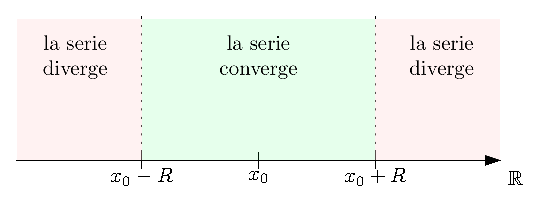
\includegraphics[width=300pt]{images/raggioConvergenza.eps}
    \caption{raggio di convergenza}
\end{figure}\acc
Essendo che nei punti $x_0-R$ e $x_0+R$ non è chiaro se una serie di potenze converga, risulta 
necessario studiarla specificatamente.
$$ 
 \text{ per }\sum_{k=0}^{+\infty}a_k(x-x_0)^k \text{ si considerano }  \begin{cases}
    \displaystyle \sum_{k=0}^{+\infty}a_kR^k \text{  }\text{ per }x_0+R  \\
   \displaystyle \sum_{k=0}^{+\infty}(-1)^ka_kR^k \text{  }\text{ per }x_0-R
 \end{cases}
$$
\subsection{Calcolo del raggio}
Data una serie di potenze, si vuole ricavare il valore del raggio $R$. A tal proposito, sarà necessario 
trovare un altro valore caratterizzante associato alla serie, che denoteremo $L$, tale $L$ non è altro 
che il valore determinante nel criterio della radice e del rapporto in valore assoluto. Sia
 $\displaystyle \sum_{k=0}^{+\infty}a_k(x-x_0)^k $ la serie di potenze in questione, si ha che 
 $$ L = \displaystyle \lim_{k\rightarrow+\infty}\frac{|a_{k+1}|}{|a_k|} 
 = \lim_{k\rightarrow+\infty}\sqrt[k]{|a_k|}$$
 Tale valore è (definizione poco rigorosa) l'inverso del raggio di convergenza, de facto\begin{itemize}
    \item $L=0\implies R=\infty$
    \item $L=\infty\implies R=0$
    \item $0<L<\infty\implies R = \dfrac{1}{L}$ 
 \end{itemize}
 \textbf{Esercizio} : Si vuole trovare $\mathcal{E}$ per la serie 
 $$ \displaystyle \sum_{k=0}^{+\infty}\frac{(2x-5)^k}{k+1}$$
 Si raccoglie $2^k$ 
 $$ \displaystyle \sum_{k=0}^{+\infty}\frac{2^k}{k+1}(x-\frac{5}{2})^k $$
 Si ottengono coefficiente e centro, rispettivamente $a_k=\frac{2^k}{k+1}$ e $x_0 = \frac{5}{2}$. Si 
 calcola $L$ applicando il criterio della radice 
 $$ L =\displaystyle \lim_{k\rightarrow+\infty}\sqrt[k]{\frac{2^k}{k+1}}  
 = \lim_{k\rightarrow+\infty}\frac{2}{\sqrt[k]{k+1}}=2$$
 Si ha che $R=\dfrac{1}{2}$ e la serie converge per $|x-x_0|<\dfrac{1}{2}$. Si studia la serie 
 nei punti critici  $x_0-R=2$  e  $x_0+R=3$
 $$ 
 \displaystyle \sum_{k=0}^{+\infty}\frac{(2x-5)^k}{k+1}\text{ diventa }  \begin{cases}
    \displaystyle \sum_{k=0}^{+\infty}\frac{(6-5)^k}{k+1} \text{  }\text{ per }x_0+R=3  \\
   \displaystyle \sum_{k=0}^{+\infty}\frac{(4-5)^k}{k+1}\text{  }\text{ per }x_0-R=2
 \end{cases}
 $$
 La convergenza risulta essere 
 $$ 
 \begin{cases}
    \displaystyle \sum_{k=0}^{+\infty}\frac{(6-5)^k}{k+1} =\displaystyle \sum_{k=0}^{+\infty}\frac{1^k}{k+1}\text{ diverge}\\
   \displaystyle \sum_{k=0}^{+\infty}\frac{(4-5)^k}{k+1}=\displaystyle \sum_{k=0}^{+\infty}\frac{(-1)^k}{k+1}\text{ converge per Leibnitz}
 \end{cases}
 $$
 A questo punto si ha l'insieme di convergenza $\mathcal{E}=[2,3)$.\acc 
 \textbf{Esercizio} :  Si vuole trovare $\mathcal{E}$ per la serie 
 $$ \displaystyle \sum_{k=0}^{+\infty}\frac{(y^2-1)^{2k}}{k+1} $$
 Si noti come non è una serie di potenze, si applica una sostituzione definendo 
 $x=(y^2-1)^2$, riscrivendo la serie come $$ 
 \displaystyle \sum_{k=0}^{+\infty}\frac{x^{k}}{k+1}$$
 Si ottengono coefficiente e centro, rispettivamente $a_k=\frac{1}{k+1}$ e $x_0 = 0$. Si 
 calcola $L$ applicando il criterio della radice 
 $$ L =\displaystyle \lim_{k\rightarrow+\infty}\frac{a_{k+1}}{a_l}=\displaystyle 
 \lim_{k\rightarrow+\infty}\dfrac{\frac{1}{k+2}}{\frac{1}{k+1}}=1\implies R=1$$
 Si studia la serie 
 nei punti critici   $x_0-R=-1$  e $x_0+R=1$
 $$ 
 \displaystyle \sum_{k=0}^{+\infty}\frac{x^{k}}{k+1}\text{ diventa }  \begin{cases}
    \displaystyle \sum_{k=0}^{+\infty}\frac{1}{k+1} \text{  }\text{ per }x_0+R=1 \text{ diverge }\\
   \displaystyle \sum_{k=0}^{+\infty}\frac{(-1)^{k}}{k+1}\text{  }\text{ per }x_0-R=-1\text{ converge }
 \end{cases}$$
 Ricordando che  $x=(y^2-1)^2$, si trova la convergenza della serie iniziale risolvendo 
 la disequazione
 $$ -1\le (y^2-1)^2= <1\begin{cases}
    -1\le (y^2-1)^2\text{ sempre vero }\\ (y^2-1)^2<1\implies y^2-1<1\implies y<\sqrt{2}
 \end{cases}$$
 Si ha quindi che $\mathcal{E}=(-\sqrt{2},\sqrt{2})\backslash\{0\}$.\acc
 \prop{} Sia $f$ una funzione derivabile infinite volte, definita come serie di potenze 
 $$ f(x)=\displaystyle \sum_{k=0}^{+\infty}a_k(x-x_0)^k $$
 si ha che \eqImportante{$f^{(k)}(x_0)=k!\cdot a_k$}
 \chapter{Integrali}
\end{document}
